\chapter*{Introduction}
\addstarredchapter{Introduction}
\renewcommand\chapterillustration{INT/INT}
\ThisULCornerWallPaper{1}{\chapterillustration}

\lettrine[lines=4, slope=-0.5em,nindent=10pt]{L}{e} détecteur \textit{Compact Muon Solenoid} (CMS) est un détecteur généraliste placé sur la ligne du faisceau du collisionneur \textit{Large Hadron Collider} situé à l'Organisation Européenne pour la Recherche Nucléaire (CERN). CMS a permis de produire d'excellents résultats scientifiques\footnote{Plus de \num{600} papiers ont été publiés.} et notamment la découverte du boson de \bsc{Higgs} en \num{2012} (cf.Fig~\ref{higgs}) conjointement avec le détecteur \textit{A Toroidal LHC ApparatuS} (ATLAS). 
\vspace*{-0.4cm}
\begin{figure}[ht!]
	\centering
	\subfloat[Distribution de la masse invariante en diphoton. Chaque événement est affecté du poids $S/(S+B)$ de sa catégorie. Les lignes représentent l'ajustement du bruit de fond et du signal, les bandes colorées représentent les écarts-types du bruit de fond à $\pm 1$ et $\pm 2 \sigma$.]{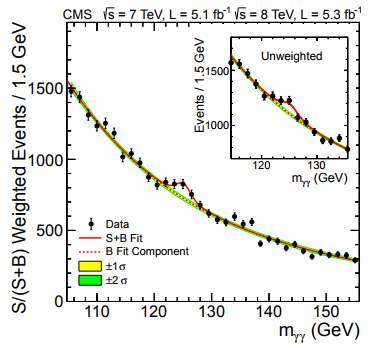
\includegraphics[width=0.49\textwidth]{INT/higgs1.png}}
	\hfill
	\subfloat[Distribution de la masse invariante pour l'analyse $ZZ\rightarrow4l$. Les points représentent les données, les histogrammes pleins le bruit de fond et l'histogramme creux montre le signal attendu pour un boson de \bsc{Higgs} de masse $M_{H}=\SI{125}{\giga\eV}$ ajouté au bruit de fond attendu.]{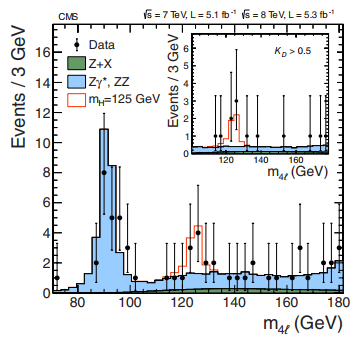
\includegraphics[width=0.49\textwidth]{INT/higgs2.png}}
	\caption{Les deux canaux de désintégration du boson de \bsc{Higgs} ayant permis sa découverte dans l'expérience CMS \cite{Chatrchyan:2012xdj}.}
	\label{higgs}
	\vspace*{-0.3cm}
\end{figure}

Cependant, aucune trace de nouvelle physique n'a été trouvée. Afin d'améliorer la capacité de détection de nouvelle physique, le LHC va subir une mise à niveau en \num{2026} afin d'augmenter sa luminosité instantanée par un facteur \num{5} à \num{7.5} et sera renommé pour l'occasion \textit{High Luminosity Large Hadron Collider} (HL-LHC). L'augmentation de la luminosité du LHC aura des conséquences importantes pour les détecteurs placés sur sa ligne de faisceaux (augmentation de l'empilement et du flux de particules produites lors des collisions etc.). Afin de faire face à l'augmentation du taux de collisions et de profiter de cette augmentation de luminosité instantanée, le détecteur CMS doit être mis à niveau. 

Cette thèse se concentre sur la mise à niveau du trajectographe à muons de CMS et plus particulièrement sur l'instrumentation de zones de ce trajectographe par des Resistive Plate Chambers (RPC) de nouvelle génération capables de supporter les flux de particules parcourant ces zones. 

Le premier chapitre décrit succinctement le contexte historique, théorique et expérimental de la physique des particules et présente également ses lacunes. Ceci nous permettra de comprendre les enjeux et la nécessité de construire des collisionneurs et des détecteurs de plus en plus puissants.

Le second chapitre présente le LHC, le collisionneur le plus puissant actuellement, sa chaine d'accélération nécessaire pour porter à une énergie inégalée jusqu'alors, les différentes expériences placées sur sa ligne de faisceaux et le projet de sa mise à niveau vers le HL-LHC.

Le troisième chapitre décrit de manière détaillée le détecteur CMS ainsi que l'ensemble de ses sous-détecteurs. Il présente également le système de déclenchement et d'acquisition de données ainsi que plusieurs des améliorations nécessaires pour sa mise à niveau afin de pouvoir profiter au maximum de la hausse de la luminosité instantanée qui sera fournie par le HL-LHC.

Le quatrième chapitre se veut un historique sommaire des RPC ainsi qu'une explication de leur principe et leurs modes de fonctionnement en général. Il décrit également les chambres RPC présentes dans CMS, le mélange de gaz utilisé, leur électronique et la détermination de leurs points de fonctionnement. Il présente aussi les améliorations qui seront apportées lors de la mise à niveau du trajectographe à muons ainsi que le type de chambre et d'électronique privilégié pour cette mise à niveau.

Le cinquième chapitre présente les résultats obtenus lors de divers tests en faisceaux à DESY (Allemagne), au PS, SPS, GIF++ (tous trois basés au CERN), pour un type de chambre, utilisant des verres de basse résistivité, développé à l'IPNL en collaboration avec nos collègues chinois de l'Université de Tsinghua. Il présente également les types d'électronique utilisés lors de ces tests en faisceaux et les programmes d'analyse utilisés afin d'obtenir ces résultats ainsi que leur validation par simulation Monte-Carlo. Il démontre également la faisabilité de grandes chambres de type RE1/1 en utilisant des verres de taille maximale \SI{32}{\centi\meter}$\times$\SI{30}{\centi\meter} et ce par deux méthodes différentes de pavage.

Le sixième chapitre présente un prototype de PCB à strips ainsi qu'une électronique à base d'ASIC PETIROC2 permettant d'obtenir la position le long des strips par lecture de ceux-ci des deux côtés. Les tout premiers résultats obtenus avec ce PCB, qui ont permis de choisir et de privilégier cette solution pour le TDR concernant la mise à niveau du trajectographe à muons de CMS, sont également inclus dans ce chapitre.

Le dernier chapitre fait un résumé des résultats obtenus et des démarches effectuées lors de cette thèse et expose les prochaines étapes à réaliser afin d'inclure cette électronique au sein du détecteur CMS.

Enfin, précisons pour le lecteur aussi peu enclin que l'auteur de cette thèse à la résolution des énigmes engendrées par l'utilisation de sigles  et d'acronymes qu'un glossaire répertoriant ces termes abscons est placé en fin d'ouvrage.


